\documentclass{beamer}

\usetheme{MagdeburgFIN}
\usefonttheme{structurebold}
\usepackage{graphicx}
\usepackage{float}
\usepackage{url}
\usepackage{pdfpages}
\usepackage{xfrac}
\usepackage[export]{adjustbox}
\usepackage{wrapfig}
\usepackage{verbatim}

\setbeamertemplate{caption}[numbered]

\title{MS-III. Implementation}
\author{Ali Hashaam, Ali Memon, Guzel Mussilova, Pavlo Shevchenko}
\date{June 13, 2017}
\institute{Scientific Project: Databases for Multi-Dimensional Data, Genomics and Modern Hardware}

\begin{document}

\begin{frame}[plain]
 \titlepage
\end{frame}

\begin{frame}
\frametitle{Table of Contents}
\tableofcontents 
\end{frame}

\section{Blinktopus}
\begin{frame}
\frametitle{Our Goal}
To provide a \textbf{framework} that gives user a chance to act as \textit{Holistic SV Optimizer} like in OctopusDB \\
Add \textbf{Approximate Query Processing (AQP)} techniques\\
\textbf{Evaluate} performance depending on choice of SV
\end{frame}


\section{Recall}
\begin{frame}
\frametitle{Building a Blinktopus. Recall}
First, the Octopus:
\begin{itemize}
\item{Store incoming data in logs.}
\item{Query the logs (just a filter query).}
\item{Allow users to create views (row, column) over certain logs.}
\item{List all views and logs.}
\item{Launch the query over views or over logs, see the changes in performance.}
\end{itemize}
\end{frame}


\begin{frame}
\frametitle{Building a Blinktopus. Recall}
Enters Approximate Query Processing (AQP):
\begin{itemize}
\item{Which synopsis will we choose to test? (Samples, histograms, sketches?)}
\item{Do Octopuses and AQP match well together?}
\item{Build the selected synopsis on the whole data, after data insertions.}
\item{Using the synopsis, answer the user queries by reconstructing the approximate data.}\\
\end{itemize}
\end{frame}


\section{Implementation}

\begin{frame}
%\frametitle{Building a Blinktopus. Implementation}
\hspace{0.2 cm} \textbf{\fontsize{14}{12}\selectfont Building a Blinktopus. Implementation}
\end{frame}

\subsection{Schema}
\begin{frame}
\frametitle{Schema}
\begin{figure}
  \centering
  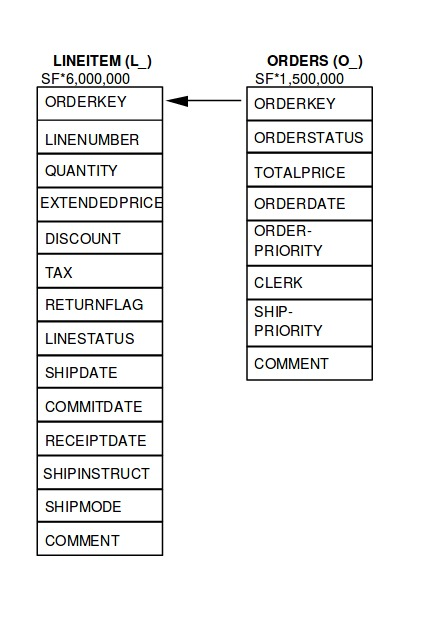
\includegraphics[scale=0.33]{img/Blinktopus-Schema.jpg}
  \caption{TPC Standard Schema}
\end{figure}
\end{frame}

\subsection{OctopusDB}
\begin{frame}
\frametitle{OctopusDB. Customization/Alteration/Power to User/Variation}
\begin{figure}
\centering
\begin{minipage}{.5\textwidth}
  \centering
  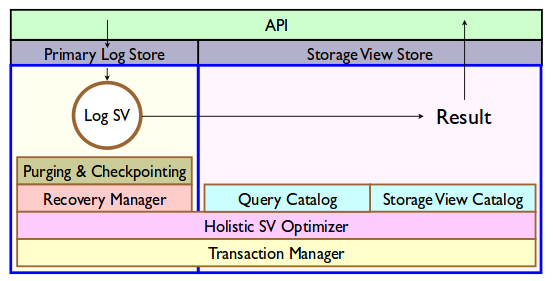
\includegraphics[scale=0.25]{img/octopus_arch.png}
  \caption{OctopusDB Architecture.}
\end{minipage}%
\pause
\begin{minipage}{.5\textwidth}
  \centering
  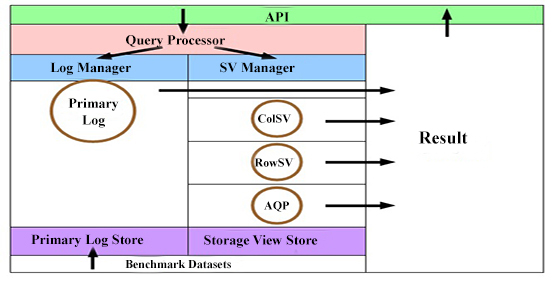
\includegraphics[scale=0.25]{img/Blinktopus-OctopusPart.jpg}
	\caption{Blinktopus.}
\end{minipage}
\end{figure}
\end{frame}

\begin{frame}
\frametitle{OctopusDB. Evaluation}
\begin{figure}
  \centering
  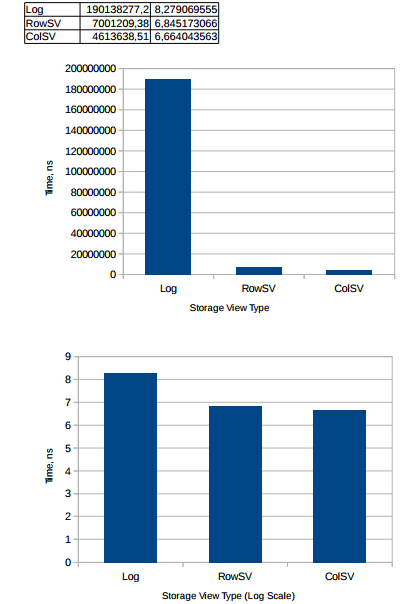
\includegraphics[scale=0.5]{img/Blinktopus-Evaluations.png}
  \caption{Evaluation result for 100 runs over Totalprice Column in Orders with Range from 50,000 to 200,000.}
\end{figure}
\end{frame}

\subsection{Approximate Query Processing}
\begin{frame}
\frametitle{AQP. Synopses}
4 main families of synopses\footnote{\tiny Cormode, Graham, Minos Garofalakis, Peter J. Haas, and Chris Jermaine. "Synopses for massive data:
Samples, histograms, wavelets, sketches." Foundations and Trends in Databases 4, no. 1–3 (2012): 1-294.}:
\begin{itemize}
\vspace{0.3 cm}
\item{Samples}
\item{Histograms \checkmark}
\item{Wavelets}
\item{Sketches \checkmark}
\end{itemize}
\end{frame}
\subsubsection{Histograms}
\begin{frame}
\frametitle{AQP. Histograms}
	In histogram's development, main cornerstones are:
	\begin{itemize}
		\item {Partition the dataset into buckets.}
		\item {Store summary statistics for each bucket about the data values in the it.}
		\item {Store information about the buckets themselves, like bucket boundaries.}
	\end{itemize}
	At query time, the summary and bucket information is used to approximately answer the query.
\end{frame}

\begin{frame}
\frametitle{AQP. Histograms}
	Vital Points to consider:
	\begin{itemize}
		\item Bucketing Scheme
		\item Statistics Stored per Bucket
		\item Approximation Scheme
		\item Class of queries answered		
		\item Efficiency
		\item Accuracy \& Error Estimates
		\item Incremental Maintenance
	\end{itemize}
\end{frame}

\begin{frame}
\frametitle{AQP. Histograms}
\begin{figure}
  \centering
  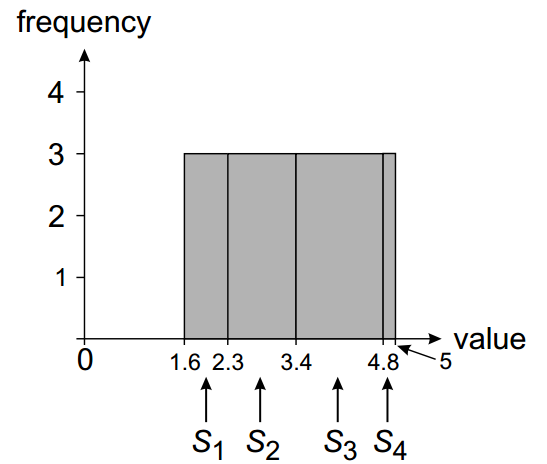
\includegraphics[scale=0.3]{img/Blinktopus-EquiDepth.png}
  \caption{Equi-Depth Histogram} 
  %\footnote{Cormode, Graham, Minos Garofalakis, Peter J. Haas, and Chris Jermaine. "Synopses for massive data: Samples, histograms, wavelets, sketches." Foundations and Trends in Databases 4, no. 1–3 (2012): 1-294.}
\end{figure}

To calculate number of bins 'k':\\
	\hspace{1 cm} $k = 2n^{\sfrac{1}{3}}$ \hspace{0.4 cm} (RICE RULE)
%	\footnote{Rice Rule: http://onlinestatbook.com/2/graphing_distributions/histograms.html}

\end{frame}

\begin{frame}
\frametitle{AQP. Histograms}
What if the count of the values between 1.1 and 4.5 is required?\\
\begin{figure}
  \centering
  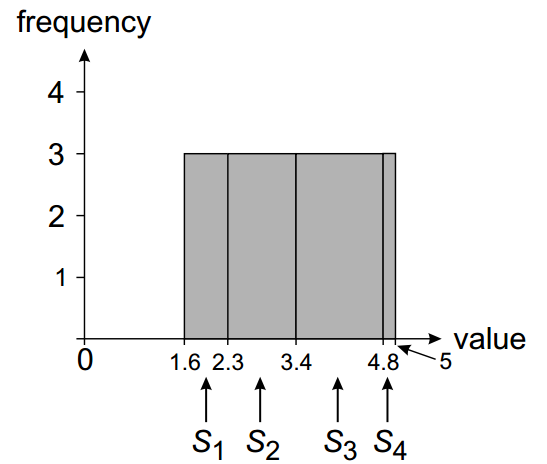
\includegraphics[scale=0.30]{img/Blinktopus-EquiDepth.png}
\end{figure}
Continuous value Assumption allows the estimation of values inside a bucket via interpolation. \\
\vspace{0.3 cm}
$ N = 3 + 3 + ((4.5 − 3.4)/(4.8 − 3.4))3 = 8.4$
\end{frame}

\begin{frame}
\frametitle{AQP. Histograms}
	\begin{itemize}
		\item Histograms are a natural solution for range-sum and range-count queries.
		\item Conceptual simple and relatively simple in interpretation.
		\item Practically acceptable accuracies, provided that the sufficient storage space are allocated.
	\end{itemize}
\end{frame}

\begin{frame}
\frametitle{AQP. Histograms}
	\begin{itemize}
		\item Sensitive to dimensionality.
		\item Performance strongly depends on bucketing schemes(how the buckets are chosen, what statistics are stored, how estimates are extracted, and what classes of query are supported).
		\item Incremental maintenance.
		\item Might provide too loose error estimates over the class of queries.
	\end{itemize}
\end{frame}

\subsubsection{Sketches}
\begin{frame}
\frametitle{AQP. Sketches}

\end{frame}

\begin{frame}
\frametitle{AQP. HLL}

\end{frame}

\begin{frame}
\frametitle{Building a Blinktopus. IDE}
\begin{itemize}
\item{Back end}
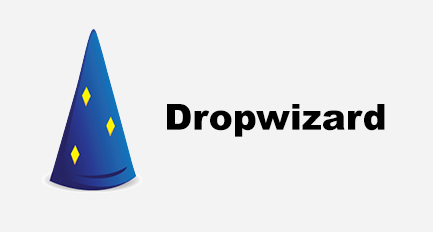
\includegraphics[scale=0.3]{img/dropwizard.png}
\vspace{0.25 cm}
\item{Front end}

\includegraphics[scale=0.2]{img/jpnotebook.png}
\footnote{\tiny 
Sources: http://jupyter.org/\\
http://honstain.com/new-dropwizard-1-0-5-java-service/}
\end{itemize}
\end{frame}

\section{Project Organisation}

\subsection{Roles}
\begin{frame}
\frametitle{Project Organisation.Roles}
\textbf{Team:} \\
\hspace{0.3 cm}Guzel - Team Leader-Researcher\\
\hspace{0.3 cm}Pavlo - Developer (Backend - OctopusDB)\\
\hspace{0.3 cm}Ali H. - Developer (Backend - AQP)\\
\hspace{0.3 cm}Ali M. - Developer (Frontend - User Views)\\
\vspace{0.2 cm}
\textbf{Supervisor:} \\
\hspace{0.3 cm} Gabriel Campero Durand \\
\vspace{0.2 cm}
Changing roles after each milestone.
\\ \vspace{0.5 cm}
\textbf{Meetings:} \\ 
\hspace{0.5 cm} Team Meetings: Mo 14-15 \\
\hspace{0.5 cm} Meetings with supervisor: We 10-11
\end{frame}

\begin{frame}
 \frametitle{Thank you! Any questions?}
\end{frame}

\section{Literature}
\begin{frame}
\frametitle{Literature}
\begin{enumerate}
\item{Jindal, Alekh. "The mimicking octopus: Towards a one-size-fits-all database architecture." VLDB PhD Workshop. 2010.}
\item{Dittrich, Jens, and Alekh Jindal. "Towards a One Size Fits All Database Architecture." CIDR. 2011.}
\item{Jindal, Alekh. "OctopusDB: flexible and scalable storage management for arbitrary database engines." (2012).}
\item{Mozafari, Barzan, and Ning Niu. "A Handbook for Building an Approximate Query Engine." IEEE Data Eng. Bull. 38, no. 3 (2015): 3-29.}
\item{Cormode, Graham, Minos Garofalakis, Peter J. Haas, and Chris Jermaine. "Synopses for massive data: Samples, histograms, wavelets, sketches." Foundations and Trends in Databases 4, no. 1–3 (2012): 1-294.}
%%\item{https://yahooeng.tumblr.com/post/135390948446/data-sketches}
\end{enumerate}
\end{frame}

\end{document}
